Un mundo se compone de varias zonas, cada una con su propio diseño, temática y desafíos. Las zonas pueden incluir 
distintos tipos de terreno, estructuras, enemigos y recursos, lo que permite a los jugadores experimentar una gran 
variedad de entornos y situaciones dentro de un mismo mundo. Más adelante se detalla cómo es posible viajar de una 
zona a otra.

\vspace{0.05cm}

Para facilitar su edición, en el creador de mundos, se implementó un \textit{editor de zonas} que permite configurar visualmente las texturas del suelo y el cielo.
Los creadores pueden seleccionar entre distintas texturas predeterminadas (Asumiendo que el mismo ya importó el contentido predeterminado que se verá más adelante) 
ó importar sus propias texturas personalizadas que serán reflejadas en el juego

\vspace{0.25cm}

Para la textura del suelo, se puede configurar la granularidad del mismo,
lo que determina la escala de repetición de la textura y permite ajustar su apariencia para adaptarse mejor a la composición visual de la zona. 

\begin{figure}[H]
\centering
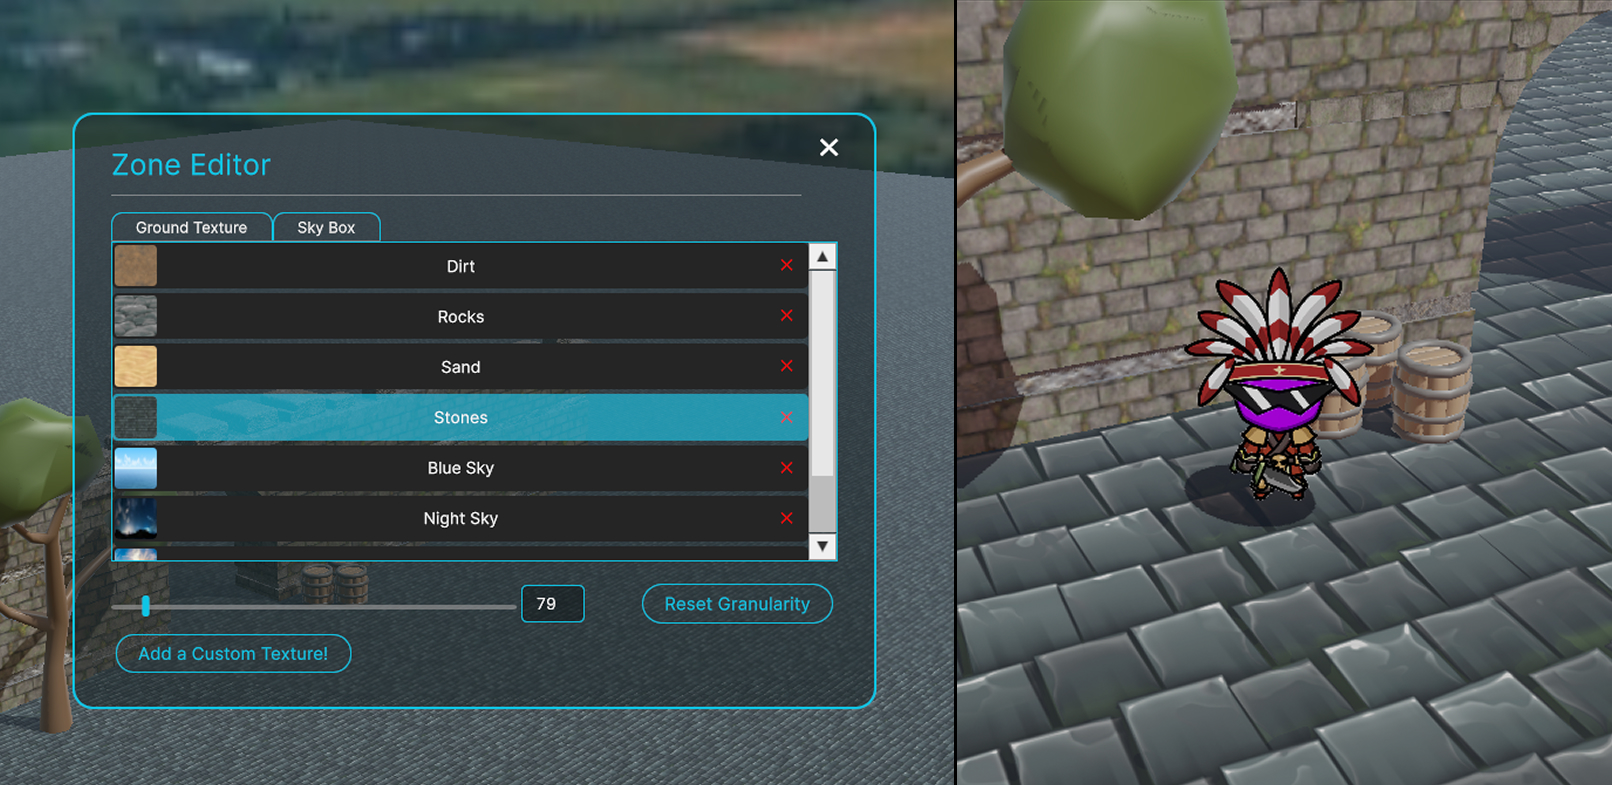
\includegraphics[width=\textwidth]{img/08-implemented-solution/product/zone-editor.jpg}
\caption{Captura de una zona con las texturas editadas.}
\label{fig:zone-editor}
\end{figure}